\documentclass[11pt,a4paper]{article}
\usepackage[top=3cm, bottom=2cm, left=2cm, right=2cm]{geometry}
\usepackage[utf8]{inputenc}
\usepackage{amsmath, amsfonts, amssymb}
\usepackage{siunitx}
\usepackage[brazil]{babel}
\usepackage{graphicx}
\usepackage[margin=10pt,font={small, it},labelfont=bf, textfont=it]{caption}
\usepackage[dvipsnames, svgnames]{xcolor}
\DeclareCaptionFont{MediumOrchid}{\color[svgnames]{MediumOrchid}}
\usepackage[pdftex]{hyperref}
\usepackage{natbib}
\bibliographystyle{plainnat}
\bibpunct{\textcolor{MediumOrchid}{\textbf{[}}}{\textcolor{MediumOrchid}{\textbf{]}}}{,}{s}{}{}
\usepackage{color}
\usepackage{footnote}
\usepackage{setspace}
\usepackage{booktabs}
\usepackage{multirow}
\usepackage{subfigure}
\usepackage{fancyhdr}
\usepackage{leading}
\usepackage{indentfirst}
\usepackage{wrapfig}
\usepackage{mdframed}
\usepackage{etoolbox}
\usepackage[version=4]{mhchem}
\usepackage{enumitem}
\usepackage{caption}
\usepackage{titlesec}
\usepackage{tcolorbox}
\usepackage{tikz}
\usepackage{LobsterTwo}
\usepackage[T1]{fontenc}
\usepackage{fontspec}
\usepackage{txfonts}
\usepackage[bottom]{footmisc}
\tcbuselibrary{skins,breakable}
\sisetup{output-decimal-marker={.}}

\makeatletter
\def\footnoterule{\kern-3pt\color{MediumOrchid}\hrule\@width0.6\textwidth height 0.8pt\kern2.6pt}
\makeatother

\renewcommand{\footnotelayout}{\itshape\color{MediumOrchid}}

\AtBeginEnvironment{equation}{\fontsize{13}{16}\selectfont}


\titleformat{\section}{\LobsterTwo\huge\color{CarnationPink}}{\thesection.}{1em}{}
\titleformat{\subsection}{\LobsterTwo\huge\color{CarnationPink}}{\thesubsection}{1em}{}
\titleformat{\subsubsection}{\bf\LobsterTwo\Large\color{MediumOrchid}}{\thesubsubsection}{1em}{}


\DeclareCaptionLabelFormat{figuras}{\textcolor{DarkTurquoise}{Figura \arabic{figure}}}
\captionsetup[figure]{labelformat=figuras}

\makeatletter
\renewcommand\tagform@[1]{\maketag@@@{\color{CarnationPink}(#1)}}
\makeatother

\renewcommand{\theequation}{Eq. \arabic{equation}}
\renewcommand{\thefigure}{Fig. \arabic{figure}}
\renewcommand{\thesection}{\textcolor{CarnationPink}{\arabic{section}}}

\setlist[itemize]{label=\textcolor{CarnationPink}{$\blacksquare$}}

\setlist[enumerate]{label=\textcolor{CarnationPink}{\arabic*.}, align=left, leftmargin=1.5cm}


\newcounter{exemplo}

\NewDocumentEnvironment{exemplo}{ O{} }{%
\allowbreak
\setlength{\parindent}{0pt}
  \begin{mdframed}[
  leftline=true,
  topline=false,
  rightline=false,
  bottomline=false,
  linewidth=2pt,
  linecolor=CarnationPink,
  frametitlerule=false,
  frametitlefont=\LobsterTwo\large\color{CarnationPink},
  frametitle={\color{CarnationPink}\LobsterTwo\large #1},
  ]
}{%
  \end{mdframed}
}

\setlength{\fboxsep}{5pt}
\setlength{\fboxrule}{1.5pt}
\usepackage{float}
\renewcommand{\thefootnote}{\alph{footnote}}
\usepackage{url}
\hypersetup{
	colorlinks=true,
	linkcolor=DarkTurquoise,
	filecolor=DarkTurquoise,      
	urlcolor=DarkTurquoise,
	citecolor=DarkTurquoise,
	pdftitle={Especialista em Física da Radioterapia}
}
\pagestyle{fancy}
\fancyhf{}
\renewcommand{\headrulewidth}{0pt}
\rfoot{\color{DarkTurquoise}\thepage \\ \LobsterTwo{\small\textcolor{CarnationPink}{@defDalila}}}

\title{\LobsterTwo\Huge{Exercícios}}
\author{\LobsterTwo\Large{Radiações Ionizantes e Dose Absorvida}\nocite{*}}
\date{\LobsterTwo\textit{Dalila Mendonça}}
\begin{document}
	\maketitle

\begin{exemplo}[Radiação Ionizante]
    \textcolor{MediumOrchid}{\LobsterTwo\textbf{Interação de Fótons}}
    \begin{itemize}
        \item Os cinco principais tipos de interações de fótons com a matéria em ordem de limiar de energia são (1) espalhamento de Rayleigh, também conhecido como espalhamento coerente, espalhamento clássico ou espalhamento elástico; (2) efeito fotoelétrico, também conhecido como absorção fotoelétrica; (3) espalhamento Compton, também conhecido como espalhamento incoerente, ou efeito Compton; (4) produção de pares; e (5) fotodesintegração nuclear ou Efeito fotonuclear.
        
        \item No espalhamento Rayleigh, o fóton incidente interage com o átomo como um todo, espalhando-se em uma direção diferente sem perder energia. Não ocorre ionização no espalhamento Rayleigh porque os elétrons não são ejetados.
        
        \item No efeito fotoelétrico, toda a energia do fóton incidente é transferida para um elétron orbital, que é então ejetado do átomo. A energia do elétron ejetado (fotoelétron) é a energia do fóton incidente menos a energia de ligação. A emissão de raios-X característicos ou elétrons Auger ocorrerá subsequentemente, preenchendo a lacuna do fotoelétron.
        
        \item O espalhamento Compton é uma colisão entre um fóton e um elétron orbital de camada externa fracamente ligado de um átomo, resultando em um fóton espalhado de menor energia e um elétron com determinada energia cinética. Esta é a interação dominante dos feixes de raios X terapêuticos com o tecido. Como a energia do fóton incidente excede em muito a energia de ligação do elétron da camada externa, a interação Compton parece uma colisão entre o fóton e um elétron livre (denominado quase livre).
        
        \item Na produção de pares, o fóton interage fortemente com o campo eletromagnético de um núcleo atômico e perde toda a sua energia para criar um elétron e um pósitron.
        
        \item Na fotodesintegração, um fóton incidente com alta energia (>7 a 10 MeV) colide com o núcleo de um átomo e toda a energia do fóton é absorvida. O núcleo então emite um nêutron. Este efeito causa requisitos extras de blindagem para feixes de alta energia.
        
        \item Com um fóton de entrada, as partículas de saída produzidas pelas quatro interações de fótons são listadas a seguir:
            \begin{enumerate}[label=\roman*.]
                \item Espalhamento Rayleigh: um fóton;
                \item Efeito fotoelétrico: um elétron;
                \item Espalhamento Compton: um elétron e um fóton;
                \item Produção de pares: um elétron e um pósitron.
            \end{enumerate}

        \item O efeito fotoelétrico é proporcional a $Z^3/E^3$, onde Z é o número atômico do átomo alvo e E é a energia do fóton incidente.
        
        \item A probabilidade de espalhamento Compton é independente de Z e diminui com E. O espalhamento Compton depende da densidade eletrônica$N_e$ do material.
        
        \item A probabilidade de produção de pares muda com $Z^2$ e log(E).
        
        \item O espalhamento Compton é mais provável de ocorrer com os elétrons da camada externa.
        
        \item A energia mínima de um fóton incidente para o processo de produção de pares é de 1,02 MeV. Essa energia corresponde à massa do elétron e do pósitron produzidos (0,511 MeV cada). A energia adicional acima do limite de 1,02 MeV é convertida em energia cinética para o par.
        
        \item O efeito fotoelétrico é a principal causa da absorção dos fótons com energia de 10 a 100 keV em água. Esta é a faixa dos raios-X de diagnóstico. A dependência da absorção do número atômico $Z^3$ fornece o excelente contraste das imagens de raios-x diagnósticas.
        
        \item O espalhamento Compton é a principal causa da absorção de fótons com energia de 100 keV–10 MeV na água. Esta é a faixa dos raios-X terapêuticos.
        
        \item O efeito fotoelétrico é mais provável quando a energia do fóton é ligeiramente maior que a energia de ligação do elétron orbital. No espectro de absorção, as energias de ligação das camadas aparecem como picos agudos conhecidos como “bordas de absorção”, rotulados pela camada correspondente, por exemplo, borda K, para absorção da camada mais interna.
        
        \item KERMA é a Energia Cinética Liberada por unidade de MAss e representa a energia transferida para o meio pelo fóton.
        
        \item As probabilidades de espalhamento Compton e efeito fotoelétrico são aproximadamente as mesmas para fótons de aproximadamente 30 keV interagindo com tecidos moles.
        
        \item No espalhamento Compton, à medida que a energia do fóton incidente aumenta, tanto os fótons quanto os elétrons são espalhados mais na direção direta. Além disso, a proporção de energia transportada pelo elétron espalhado aumenta com a energia do fóton incidente.
        
        \item No espalhamento Compton, a energia máxima do fóton espalhado é 511 keV a 90° e 255 keV a 180° (ou seja, retroespalhamento). Estas são as energias de interesse para blindagem secundária.
        
        \item Uma vacância criada na camada K causa a transição de um elétron de uma camada superior para a camada K. Isso pode criar uma vacância na camada intermediária (por exemplo, L ou M) que pode ser preenchida por um elétron de camada ainda mais alta. Essa cascata de elétrons continua à medida que os elétrons da camada externa saltam para as camadas internas. A diferença em suas energias de ligação é liberada como raios-X característicos ou elétrons Auger.
    \end{itemize}

    \textcolor{MediumOrchid}{\LobsterTwo\textbf{Interação de Partículas}}
    \begin{itemize}
        \item Partículas alfa (\ce{\alpha2+} ou \ce{He2+}), prótons (p+), partículas beta (\ce{\beta-}), pósitrons (\ce{\beta+}) e elétrons (e-) são alguns exemplos de partículas carregadas. Fótons (ou seja, raios X e raios gama), nêutrons e neutrinos são alguns exemplos de partículas sem carga.
        
        \item As partículas carregadas podem sofrer três tipos de interação: excitação, ionização e produção bremsstrahlung. Excitação e ionização são interações da partícula carregada com os elétrons orbitais. Bremsstrahlung é uma interação da partícula carregada com o núcleo.
        
        \item A principal diferença entre excitação e ionização está relacionada ao elétron orbital ser ou não ser ejetado do átomo. Na excitação, a energia transferida não excede a energia de ligação do elétron, então o elétron é elevado a um nível de energia mais alto mas ainda se mantém ligado ao átomo. Na ionização, a energia transferida excede a energia de ligação do elétron, então o elétron é ejetado do átomo.
        
        \item Raios X, raios gama, elétrons, prótons, partículas alfa e nêutrons são alguns exemplos de radiação ionizante. Microondas, ondas de rádio e fótons ópticos são alguns exemplos de radiação não ionizante.
        
        \item A radiação diretamente ionizante vem de partículas carregadas (por exemplo, prótons, elétrons e partículas alfa) e a radiação indiretamente ionizante vem de partículas não carregadas (por exemplo, fótons e nêutrons).
        
        \item Os raios delta são elétrons secundários com energia suficiente para percorrer uma distância significativa do feixe de radiação primário e produzir mais ionização (ou seja, ionização secundária).
        
        \item O número médio de pares de íons primários e secundários produzidos por unidade de comprimento do caminho da partícula carregada é chamado de Ionização Específica (IS). O SI geralmente é expresso em unidades de pares de íons por mm (par de ions/mm).
        
        \item A  Ionização Específica aumenta com $Q^2$ e diminui com $v^2$. Assim, $IS \propto Q^2/v^2$.
        
        \item À medida que um próton viaja através da matéria, ela perde velocidade, fazendo com que sua ionização específica (IS) aumente até um máximo, chamado de pico de Bragg, quando ela para definitivamente. A ionização específica cai rapidamente depois que o próton deposita sua energia.
        
        \item O comprimento do caminho de uma partícula é a distância que a partícula percorre, enquanto o alcance de uma partícula é a profundidade de penetração da partícula na matéria. O comprimento do caminho percorrido de um elétron individual quase sempre excede seu alcance, enquanto o comprimento do caminho percorrido de uma partícula carregada pesada (por exemplo, partículas alfa) é essencialmente igual ao seu alcance.
        
        \item A LET é a quantidade média de energia depositada localmente na matéria por unidade de comprimento do caminho. A LET é frequentemente expressa em unidades de keV por \unit{\mu m} (\unit{keV/\mu m}).
        
        \item O LET de uma partícula carregada aumenta com $Q^2$ e diminui com $E_k$. Assim, $LET \propto Q^2/E_k$
        
        \item Partículas alfa, prótons e nêutrons são exemplos de radiação com alta LET. Elétrons, raios X e raios gama são exemplos de radiações de baixa LET.
        
        \item À medida que um elétron interage com um núcleo atômico, ele é desviado de sua trajetória e desacelerado pelo núcleo carregado positivamente, com perda de energia cinética que leva a emissão de raios-X bremsstrahlung. Bremsstrahlung é uma palavra alemã que significa ``radiação de freamento''.
        
        \item A emissão total de bremsstrahlung por átomo aumenta com $Z^2$ e diminui com $m^2$. Assim, bremsstrahlung $\propto Z^2/m^2$.
        
        \item Um pósitron interage com um elétron no final de seu alcance, resultando na aniquilação do par elétron-pósitron e na conversão de sua massa de repouso em energia na forma de dois fótons de 0,511 MeV com direções opostas.
        
        \item O poder de freamento de uma partícula carregada é a perda de energia por unidade de comprimento de caminho em um meio, geralmente dado em unidades de MeV/m ou joule (J/m).
        
        \item O poder de freamento mássico de uma partícula carregada é o poder de freamento dividido pela densidade do meio, geralmente dado em unidades de MeV m2/kg ou J m2/kg.
        
        \item De acordo com o destino da energia perdida pela partícula carregada, o poder de freamento pode ser dividido em “poder de freamento de colisão”, resultado da excitação e ionização e “poder de freamento radiativa”, resultado da produção bremsstrahlung.
        
        \item Analisando a velocidade relativa das partículas alfa, prótons e elétrons com a mesma energia cinética, a velocidade da partícula $\alpha^{2+} < p^{+} < e^{-}$. A energia cinética depende da massa e do quadrado da velocidade. Para a mesma energia, a partícula mais leve será a mais rápida, então a classificação segue a massa das partículas.
        
        \item Analisando o alcance relativo das partículas alfa, prótons e elétrons com a mesma energia cinética, o alcance da partícula $\alpha^{2+} < p^{+} < e^{-}$. O alcance é proporcional à massa e inversamente proporcional ao quadrado da carga elétrica.
        
        \item Os feixes prótons e as partículas carregadas pesadas usados em tratamentos permitem concentrar a dose dentro do tumor enquanto as doses no tecido sadio aos arredores do tumor é minimizada. Isto ocorre devido às caracteristicas de interação destas partículas. A medida que as partículas carregadas são desaceleradas, elas liberam mais energia no meio, e esta propriedade causa o pico de bragg, caracterizado como uma grande deposição de energia no final do alcance da partícula. 
        
        \item Os dois principais tipos de interações de nêutrons com a matéria são o espalhamento e a absorção. Os nêutrons podem interagir com os núcleos por meio de espalhamento em colisões semelhantes a “bolas de bilhar”, produzindo núcleos de recuo que depositam sua energia por meio de excitação e ionização. Os nêutrons também podem ser absorvidos por núcleos e causar uma variedade de emissões, como raios gama, partículas carregadas, nêutrons ou fragmentos de fissão.
        
        \item Os nêutrons não causam excitação e ionização diretamente. Como os nêutrons são partículas sem carga eles não interagem com os elétrons via excitação e ionização.
        
        \item O efeito Cerenkov ocorre quando uma partícula carregada viaja em um meio a uma velocidade maior que a velocidade da luz nesse meio (nenhuma partícula massiva pode viajar mais rápido que a luz no vácuo). Nessa condição, a partícula carregada cria uma “onda de choque” eletromagnética, semelhante à onda de choque acústica quando um avião viaja mais rápido que a velocidade do som. A onda de choque eletromagnético aparece como uma explosão de radiação visível, conhecida como radiação de Cerenkov. Potencialmente, isso poderia ser usado para medir a posição e a intensidade da dose depositada. A probabilidade de ocorrência do efeito Cerenkov é muito pequena (muito menos de 1\%), mas alguns pacientes que recebem tratamento com elétrons perto dos olhos podem descrever a visão de anéis azulados durante o tratamento.
        
    \end{itemize}
\end{exemplo}


\begin{exemplo}[Dose Absorvida]

    \textcolor{MediumOrchid}{\LobsterTwo\textbf{Dosimetria}}
    \begin{itemize}
        \item A exposição é definida como o quociente $dQ/dm$, onde dQ é a carga total de íons de um sinal que são produzidos no ar quando todas as partículas carregadas produzidas por fótons são completamente freadas, e dm é a massa de ar dentro da qual as partículas carregadas são liberadas. 
        
        \item A definição de exposição requer que as partículas carregadas sejam completamente paradas no ar. Para feixes de megavoltagem, o alcance de partículas carregadas no ar é muito grande para que a medição da exposição seja possível.
        
        \item O roetgen( R) é a unidade de exposição. A unidade original foi definida como a quantidade de radiação que libera 1 esu (unidade eletrostática) de carga por centímetro cúbico de ar. Para expressar o roentgen em unidades SI, usamos o fator de conversão de esu para C (Coulombs) e a densidade do ar (aproximadamente 1,293 \unit{kg/m^3}). Como 1 esu  \qty{3.34e{-10}}{C}, temos
        
        $$1R = 1 \frac{esu}{cm^3} = \frac{1\;esu \times 3.34 \times 10^{-10} \frac{C}{esu}}{1\;cm^3 \times 1.293 \frac{kg}{m^3} \times \frac{m^3}{10^6 cm^3}} = 2.58 \times 10^{-4} \frac{C}{kg}$$

        \item O fator $f$ é usado para converter a exposição, que é definida apenas no ar, para a dose em um meio. É denominado o fator roentgen para rad. Para o ar, f é 0,876.
        
        \item Assumindo que o equilíbrio de partículas carregadas existe no ponto de interesse, a dose em um meio pode ser calculada a partir da exposição a partir da seguinte equação:
        
            $$D_m(cGy) = f \times X \times \frac{\Psi_m}{\Psi_{ar}}$$

        onde X é a exposição (R) e $\Psi_{m}/\Psi_{ar}$ é a razão da fluência de energia de um meio m com o ar. O fator $f$ para a agua varia de 0.88 até 0.97 dependendo da energia dos raios X.


        \item O fator $f$ é definido como:
        
            $$f = 0.876 \frac{\left(\frac{\bar{\mu}_{ab}}{\rho}\right)_m}{\left(\frac{\bar{\mu}_{ab}}{\rho}\right)_{ar}}$$

        O numerador contém o coeficiente mássico de absorção de energia para o material de interesse enquanto que o denominador contém o coeficiente mássico de absorção de energia para o ar. Diferentes materiais possuem diferentes seções de choque para as interações e portanto $f$ é inerentemente dependente do meio. O coeficiente mássico de absorção de energia também é dependente da energia do feixe incidente uma vez que diferentes processos de interação são dominantes para diferentes energias. 

        \item A dose absorvida é a energia absorvida por unidade de massa. Esta é uma quantidade física mensurável. A unidade de medida padrão para a dose absorvida é o gray (Gy), no qual é definida como 1 joule de energia absorvida por 1 kg de massa.
        
        \item A dose absorvida é um dos fatores utilizados para explicar o efeito biológico causado pela radiação no tecido. No entanto, o efeito biológico causado pela radiação também depende de outros fatores relacionados à radiação como o tipo de radiação e a taxa com o qual a radiação é entregue.
        
        \item Ao utilizar uma câmara de ionização para mensurar a dose absorvida, utiliza-se a teroria cavitária de Bragg-Gray que permite relacionar o número de ions coletados na câmara com a dose absorvida no meio no qual a câmara está inserida. 
        
        \item Segundo a teoria cavitária de Bragg-Gray, a dose absorbida no meio ao redor da câmara está relacionada com a dose no ar dentro da câmara através da razão da média dos poderes de freamento mássico do meio e do gás dentro da câmara, no qual será equivalente à razão entre a dose no meio e a dose no gás.
        
        \item Para uitilizar a teoria cavitária de Bragg-Gray para determinar a dose abvsorvida no meio através da dose em uma cavidade inserida nesse meio deve-se assumir que: Primeiro, a presença do meio da cavidade não afeta o campo de partículas carregadas porque sua espessura é pequena em comparação com o alcance de partículas carregadas que incidem sobre ele. Em segundo lugar, toda a dose no meio da cavidade é depositada pelas partículas carregadas que o atravessam.
        
        \item A difefença entre a teoria cavitária de Bragg-Gray e a Teoria cavitária de Spencer Attix é que a teoria cavitária de Spencer-Attix utiliza o poder de freamento mássico restrito com um valor de corte de $\Delta$ (normalmente 10–20 keV) para levar em consideração o efeito dos raios delta que depositam apenas parte de sua energia no volume de interesse e pode depositar energia em uma distancia além do volume em questão. Spencer-Attix é, portanto, mais preciso que Bragg-Gray.
        
        \item O Equilíbrio de Paartículas Carregadas é o conceito de que dado um volume $V$, cada partícula carregada de um sinal e energia saindo de $V$ é, em média, substituída por uma partícula carregada idêntica da mesma energia entrando em $V$.
        
        \item De acordo com o TG-51, a equação para calibração dos aceleradores lineares é:
        
            $$D_W^Q = N_{D,w}^{{}^{60}Co} M k_Q$$
        
        onde $D_W^Q $ é a dose absorvida na água medida no ponto de referência em um feixe de qualidade $Q$ (Sua unidade é Gy). $N_{D,w}^{{}^{60}Co}$ é o coeficiente de calibração para conversão da carga medida para a dose (Sua unidade é Gy/C). $M$ é a leitura do eletrômetro corrigida, em unidades de C. $k_Q$ é o fator de correção para a qualidade no qual corrige o coeficiente de calibração devido as diferenças nas qualidades do feixe entre o feixe que está sendo calibrado e o feixe de \ce{^{60}Co}.

        \item O fator de correção para temperatura e pressão dado no TG-51 é:
        
            $$k_{T,P} = \frac{760}{P} \times \frac{273.2 + T}{295.2}$$

        onde P é a pressão atmosférica em unidades de mmHg. Para P dado em unidades de kPa o fator de correção 1kPa = 7.5 mmHg deve ser utilizado. A Temperatura T dada em \unit{\celsius} é convertida para kelvin (K) adicionando 273.2; E 295.2 é a temperatura em kelvin sob as condições de referência.


        \item Para câmaras de ionização não seladas, a sua resposta pode mudar devido à variações na temperatura e pressão justamente porque a massa de ar dentro da câmara varia com a pressão e a temperatura. O fator $k_{T,P}$ corrige os desvios de temperatura e pressão das condições de referência (295,2 K e 760 mmHg) sob as quais a câmara foi calibrada.
        
        \item O protocolo TG-51 fornece um meio para calibrar a saída de um acelerador linear. O resultado é a calibração da dose em função das Unidades Monitoras (Mu's) em um ponto específico em um fantoma de água, a uma distância padrão, para um tamanho de campo de referência.
        
        \item Normalmente, a geometria de calibração é um tamanho de campo de referência de 10 cm x 10 cm, distância da fonte até a superfície da água de 100 cm e na profundidade nominal máxima da energia calibrada. A determinação da dose em outros pontos pode então ser calculada com base em fatores de saída medidos, por exemplo, razão de tecido máximo (TMR), fator de espalhamento do colimador (Sc), fator de espalhamento do phantom (Sp), razão off-axis (OAR), porcentagem de dose na profundidade (PDP), e assim por diante.
        
        \item A carga medida pelo eletrômetro depende da polaridade aplicada à câmara de ionização. Os fótons interagem não apenas com o gás na câmara de ionização, mas também com o eletrodo coletor central, ejetando elétrons no qual podem aumentar ou diminuir dependendo da polaridade aplicada à câmara de ionização. Uma corrente adicional fora da cavidade de coleta, conhecida como corrente extracameral, também pode ocorrer devido a circuitos mal blindados ou interações que ocorrem no cabo da câmara de íonização.
        
        \item A alta voltagem de uma câmara de ionização é usada para separar e coletar os íons que se formam na presença da radiação ionizante. O processo de coleta não é 100\% eficiente e alguns íons formados se recombinam antes de chegar aos eletrodos coletores, causando perda de sinal (uma vez recombinados, formam átomos com carga elétrica neutra, o qual não é acelerado pelo campo elétrico formado pela diferença de potencial aplicada na câmara).
        
        \item O fator de correção do eletrômetro, P\textsubscript{elec}, é necessário quando a câmara deionização e o eletrômetro não são calibrados como uma unidade (juntos). Este fator é fornecido por um Laboratório de Calibração de Dosimetria Credenciado (ADCL) e deve ser verificado novamente pelo ADCL a cada dois anos.
        
        \item Suponha que 1 g de água, 1 g de ar e 1 g de poliestireno absorvem cada um 1 J de energia, como a dose absorvida é definida como a energia absorvida por unidade de massa. Como cada meio absorveu a mesma quantidade de energia e também contém a mesma massa, todos recebem a mesma dose.
        
        \item Comparando um feixe de 10 MV de fótons e um feixe de 10 MeV de elétrons, a dose na pele para o feixe de elétrons é maior do que a dose para o feixe de fótons. Feixes de fótons de alta energia (>1 MV) são indiretamente ionizantes e, portanto, depositam sua dose downstream, em alguns centímetros de profundidade. Os feixes de elétrons, no entanto, são diretamente ionizantes. Os elétrons em um feixe de elétrons podem depositar uma dose significativa diretamente na superfície do paciente.
        
        \item A absorção de fótons é baseada na densidade eletrônica e no número atômico do meio. Um phantom água-equivalente deve ter a mesma densidade eletrônica (número de elétrons por \unit{cm^3} =  $3.34 \times 10^{23}$ para a água) e número atômico efetivo, Z\textsubscript{eff} = 7.42.
        
        \item KERMA é um acrônimo que significa “kinetic energy released per unit mass” “energia cinética liberada por unidade de massa”. É definido como a razão
        
            $$KERMA = \frac{dE_{tr}}{dm}$$

        onde $dE_{tr}$ é a energia cinética inicial total de todas as partículas carregadas colocadas em movimento pelos fótons em uma massa $dm$ do material. o Kerma também pode ser calculado através da equação:

            $$KERMA = \Psi \left(\frac{\bar{\mu}_{tr}}{\rho}\right)$$

        onde $\bar{\mu}_{tr}/\rho$ é coeficiente mássico médio de transferência de energia e $\Psi$ é a fluência de energia do fóton. O Kerma é expresso em unidades de J/kg. O KERMA pode ser dividido em componente de colisão (dose depositada) e radiativa (bremsstrahlung).
    \end{itemize}

    \textcolor{MediumOrchid}{\LobsterTwo\textbf{Dosímetros}}
    \begin{itemize}
        \item Um dosímetro ideal deve ser capaz de medir a dose de radiação com precisão, com a mesma sensibilidade, independentemente do tipo de radiação, energia da radiação, taxa de dose ou histórico de exposição do dosímetro.
        
        \item Um dosímetro absoluto é aquele que não precisa ser calibrado antes de ser utilizado para medir a dose absoluta. Existem três tipos comuns de dosímetros absolutos: câmaras de ionização de ar livre, dosímetros Fricke de sulfato ferroso  e calorímetros.
        
        \item As câmaras de ionização de ar livre são grandes câmaras de ionização projetadas para medir a exposição. Seu grande tamanho e limitações de energia limitam principalmente seu uso a laboratórios de padrões nacionais.
        

        \begin{center}
            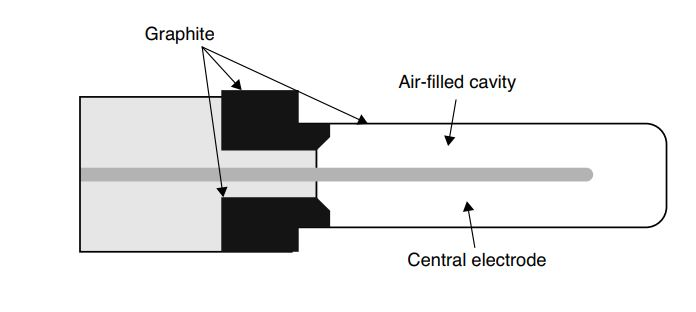
\includegraphics[width=0.4\textwidth]{Imagens/camaraDeIonização.JPG}
        \end{center}
        
        \item Uma câmara de ionização é composta por dois polos condutores e um espaço entre os polos preenchido com ar, A Radiação ioniza as moléculas de ar e forma um par elétron-íon (elétron com carga negativa e o íon com carga positiva). Essas partículas são conduzidas através de uma tensão de polarização para os dois polos da câmara e são coletadas pelo eletrômetro. O número de pares de ions produzidos e então a carga coletada nos polos é proporcional a dose de radiação recebida. A câmara de ionização é o tipo de dosímetro mais robusto para medir a dose absoluta e sua resposta é estável com respeito a taxa de dose, ou seja, a dose entregue é a mesma para a quantidade de MU entregue à diferentes taxas de dose.
        
        \item A voltagem de polarização em uma câmara de ionização é escolhida de forma que os pares de ions produzidos pela ionização direta se movam rápido o suficiente em direção aos polos de modo que não exista uma recombinação iônica significante, e ao mesmo tempo, a voltagem de polarização deve ser pequena o suficiente para que os pares de ions formados não tenham capacidade de causar mais ionizações, fazendo com que pares de ions extras sejam formados.  Normalmente é utilizada uma voltagem de polarização variando entre 150 V e 300 V (positivo ou negativo).
        
        \item A espessura da parede de uma câmara de ionização deve ser maior ou igual ao alcance das partículas secundárias carregadas (elétrons) que são produzidos na parede. Essa condição é necessária para fornecer o equilibrio eletrônico dentro do volume sensível da câmara. Em feixes de alta energia, esta condição não é satisfeita e uma capa de buil-up é necessária para fornecer uma espessura adicional à parede da câmara para manter a condição de equilíbrio eletrônico.
        
        \item A cavidade de uma câmara de ionização pode ser selada ou aberta para a atmosfera. A quantidade de ar dentro de uma câmara aberta depende da temperatura e pressão atmosférica no ponto de medida e portanto quando for realizada a medida da dose, a leitura de carga deve ser corrigida pela temperatura e pressão. Câmaras seladas fornecem uma resposta constante e não são afetadas por mudanças externas de temperatura e pressão, porém estas câmaras são vulneráveis à vazamentos.
        
        \item Uma câmara de ionização de placas paralelas também possui um volume sensível cilindrico, mas sua altura é muito menor que seu raio. Isto permite que a câmara realize medidas de um grande volume mas em uma pequena profundidade. Elas são comumente usadas para medir a dose perto da superfície de um fantoma ou na região de buil-up, além de serem utilizadas em medidas de feixes de elétrons que apresentam mudanças bruscas de dose em função da profundidade.
        
        \item As câmaras de extrapolação foram inicialmente projetadas para dosimetria de elétrons. Como câmaras de ionização têm extensão espacial finita, torna-se difícil sua utilização para medir a dose nas camadas superficiais de um meio (por exemplo, dose na superfície). As câmaras de ionização de extrapolação contêm parafusos micrométricos que são usados para ajustar o espaçamento entre seus eletrodos. A dose em um espaçamento de 0 cm pode ser extrapolada a partir de uma série de medições feitas em espaçamentos progressivamente menores. 
        
        \item Um Dosímetro Termoluminescente (TLD) é feito de materiais semicondutores que, quando expostos à radiação ionizante, permitem que os elétrons fiquem presos em estados metaestáveis (armadilhas). Quando aquecidos, esses elétrons caem no estado fundamental e a luz é liberada. A quantidade de luz liberada pelo material é então proporcional à dose de radiação. Após o aquecimento, o TLD pode ser reutilizado.
        
        \item Os materiais mais comuns utilizados na fabricação de dosímetros TLD são: 
        
            \begin{itemize}[label=\textopenbullet]
                \item \ce{LiF}:\ce{Mg},\ce{Ti}
                \item \ce{LiF}:\ce{Mg},\ce{Cu},\ce{P}
                \item \ce{Li2B4O7}:\ce{Mn}
                \item \ce{CaSO4}:\ce{Dy}
                \item \ce{CaSO4}:\ce{Mn}
            \end{itemize}
                
        \item O \ce{LiF}:\ce{Mg} é o tipo mais comum de dosímetros TLD e está disponível em várias formas incluindo pó, cartões, fitas e chips de Teflon. Este material possui uma densidade física de \qty{2.64}{g/cm^3} e número atômico efetivo $\mathrm{Z_{eff} = 8.2}$, que é perto do tecido mole onde $\mathrm{Z_{eff} = 7.4}$. O Lítio utilizado na fabricação do dosímetro pode ser o \ce{^6Li} ou o \ce{^7Li}. O \ce{^6Li} é sensível à nêutrons e o \ce{^7Li} não é sensível a nêutrons, portanto eles podem ser utilizados em combinação para determinar a componente de dose relacionada à nêutrons. 
        
        \item Ambos os \ce{CaSO4} possuem a mesma densidade física igual a \qty{2.61}{g/cm^3} e número atômico efetivo $\mathrm{Z_{eff} = 15.3}$.
        
        \item Os TLD's são um exemplo de dosímetros secundários com utilidade clínica baseados no processo de termoluminescência. A precisão destes detectores está dentro de 3\% a 5\%.
        
        \item As armadilhas de menores energias liberam seus elétrons em menos de 10 horas e, portanto, os TLDs são normalmente lidos 24 horas após a exposição para evitar a medição da luz desses elétrons. Após esse período, a precisão do TLD normalmente é mantida se os TLDs forem lidos em cerca de 12 semanas após a exposição.
        
        \item Um Dosímetro luminescente opticamente estimulado (OSLD) é semelhante a um dosímetro termoluminescente (TLD) em que a radiação do OSLD faz com que os elétrons se movam para estados metaestáveis (armadilhas). Em vez de aquecer o OSLD para fazer com que os elétrons voltem ao estado fundamental, o material é exposto a uma luz de laser verde. A luz azul emitida pelos elétrons liberados das armadilhas é proporcional à radiação absorvida pelo OSLD. A vantagem sobre o TLD é que o OSLD libera apenas 0,2\% do elétron preso, portanto, pode ser relido, se necessário. \ce{Al2O3} é o material OSL mais comum utilizado nos dosímetros.
        
        \item Um TLD é menor que um OSLD, e os TLDs têm uma dependência angular menor que os OSLDs (ou seja, resposta ao ângulo em que a radiação entra no dosímetro).
        
        \item O processo de leitura de TLDs é mais demorado e as leituras de dose dos TLDs não são instantâneas. TLDs normalmente requerem 24 horas de intervalo antes de serem lidos. OSLDs podem ser lidos instantaneamente.
        
        \item Diodos utilizados em detectores são materiais semicondutores. Na camada de depleção da junção p-n existe um campo elétrico natural. Quando a radiação ionizante atinge essa região, são criados pares elétron-buraco. Os elétrons e buracos se movem em direções opostas sob a influência da tensão de polarização natural. A carga assim coletada é proporcional à dose.
        
        \item Em comparação com as câmaras de ionização, os detectores de diodo são detectores com uma sensibilidade muito maior devido à alta densidade do material (em relação ao ar) e à pequena quantidade de energia necessária para fazer um par elétron-buraco (~ 2 eV) do que para fazer um elétron-íon par no ar (~33 eV). Portanto, eles podem ser feitos com tamanhos muito menores. Além disso, os detectores de diodo não requerem uma tensão de polarização externa uma vez que ja possuem essa tensão de polarização naturalmente. 
        
        \item Em comparação com as câmaras de ionização, os diodos são dependentes de energia e sua precisão de medição diminui quando a exposição acumulativa aumenta.
        
        \item A sensibilidade de um detector de diodo depende da taxa de dose, do espectro de energia do feixe, da direção em que a radiação entra no detector e do histórico de exposição do detector. Para usar o detector para medidas de dose absoluta, o detector deve ser calibrado com respeito a uma câmara de ionização.
        
        \item Um diodo é normalmente calibrado para fornecer a dose na profundidade nominal máxima da energia do feixe. Com uma capa de build-up, a dose relatada é normalmente a dose em dmax.
        
        \item De acordo com o TG51 apenas câmaras de ionização podem ser utilizadas para a calibração absoluta de um acelerador linear.
        
        \item O dosímetro mais utilizdo para encontrar fontes perdidas de braquiterapia é o Contador Geiger Muller devido a sua alta sensibilidade.
        
        \item Os dosimetros mais utilizados para medidas de dose in-vivo são os Diodos, TLD's, OSLDs e MOSFETS (transistores de efeito de campo semicondutores de óxido de metal).  Os dosímetros de diodo têm leituras em tempo real e são convenientes para uso diário. Eles também têm a vantagem de não precisarem de uma tensão de polarização e, portanto, são seguros para serem colocados nos pacientes. As câmaras de ionização não são usadas com frequência devido à preocupação com a alta tensão de polarização (300 V) necessária. TLDs e OSLDs não possuem leituras em tempo real. No entanto, vários detectores podem ser usados ao mesmo tempo para medições de dose em vários pontos e leitura posterior.
        
        \item As medições de vazamento (leakage) de isótopos radioativos requerem sensibilidade extremamente alta; portanto, uma câmara poço é ideal para esta tarefa.
        
        \item Um contador Geiger não pode ser utilizado para medidas em um acelerador linear pois os contadores Geiger têm um período de insensibilidade após cada liberação de radiação chamado tempo morto. Os Linacs funcionam em modo pulsado, portanto, usar um contador Geiger pode perder pulsos ou pode não responder completamente devido à alta taxa de dose envolvida.
        
        \item Os dosímetros comumente utilizados para monitoramento de exposição do IOE consistem em ``distintivos'' ou anéis contendo filmes, TLDs ou OSLDs.
        
        \item O melhor dosímetro para avaliar a distribuição de dose relativa é o filme dosimétrico. Câmaras de ionização e diodos também podem ser utilizados porém apresentam uma resolução muito menor.
        
        \item Ao ser exposto a um campo de radiação, o filme radiográfico sofre alterações químicas nos cristais de brometo de prata que causam a formação de uma imagem latente. Os processos de revelação e fixação removem grânulos de cristal não desenvolvidos deixando regiões escuras onde a radiação expôs o filme. A opacidade dessas áreas depende da quantidade de energia absorvida. Um densitômetro é usado para quantificar a densidade óptica das regiões do filme. A densidade óptica pode ser usada para quantificar a dose por meio da curva de Hurter e Driffield (H\&D).
        
        \item As principais vantagens em utilizar filmes radiográficos na dosimetria é que eles possuem alta resolução espacial e baixo custo. As principais desvantagens são que Devem ser calibrados através de uma calibração cruzada com uma câmara de ionização. O filme exibe dependência energética significativa. Bolsas de ar podem causar artefatos quando os filmes são colocados em phantoms. Fatores de correção podem ser necessários para exposições na região não linear da curva de Hurter e Driffield (H\&D). Os fótons espalhados de baixa energia interagem fortemente no filme através do efeito fotoelétrico devido à presença da prata, que tem um Z relativamente alto em comparação com os tecidos moles e ossos. Incertezas adicionais são introduzidas por diferenças nas emulsões e condições de processamento. Também requer processamento químico.
        
        \item A densidade do filme radiográfico é obtida por meio de alterações químicas nos cristais de brometo de prata. No entanto, no filme radiocrômico, a densidade é obtida por meio de um processo de polimerização. Ao contrário do filme radiográfico, o filme radiocrômico não requer processamento químico. 
        
        \item Ambos os tipos de dosimetria utilizando filme requerem a medição da densidade óptica. No filme radiográfico, a densidade óptica é medida usando um densitômetro. A medição da densidade óptica para filmes radiocrômicos requer o uso de um espectrofotômetro, microdensitômetro ou scanner a laser. O filme radiocrômico também é aproximadamente equivalente ao tecido (o filme radiográfico não é porque contém prata) e tem baixa dependência de energia e não é sensível no espectro visível.
        
        \item Os dosímetros Fricke de sulfato ferroso utilizam uma reação de oxidação que converte íons ferrosos em íons férricos. A concentração de íons férricos está relacionada com a dose absorvida. G representa o rendimento químico da radiação (número de íons férricos produzidos por 100 eV).
        
        \item Contadores proporcionais equivalentes a tecido (TEPCs), gota superaquecida, esferas de Bonner, filme de monitoramento de nêutrons, tipo A (filme NTA), trilha de fissão e detectores de albedo de dosímetro termoluminescente (TLD) podem ser usados para dosimetria de nêutrons.
        
        \item De acordo com o TG 51 As câmaras de íons devem ser calibradas assim que compradas, depois de reparadas, quando um problema é detectado e pelo menos a cada dois anos. Isso é realizado por um Laboratório de Calibração de Dosimetria Credenciado (ADCL), cujas calibrações são diretamente rastreáveis ao Instituto Nacional de Padrões e Tecnologia (NIST). O laboratório de calibração fornece a dose absorvida para o coeficiente de calibração da água para a câmara de ionização que está sendo usada. Esta calibração é denominada “diretamente rastreável” ao NIST. Uma câmara pode ser calibrada por um físico a partir de uma câmara diretamente rastreável e, então, seria “indiretamente rastreável”.
        
        \item MOSFET é um acrônimo que significa transistor de efeito de campo semicondutor de óxido de metal ``metal–oxide semiconductor field-effect transistor''. Existem quatro componentes principais de um MOSFET: um dreno, uma fonte, um gate e um substrato em massa. Em um MOSFET de canal p, uma tensão negativa é aplicada ao gate que causa um acúmulo de buracos no substrato subjacente. Quando uma tensão suficientemente grande é aplicada aogate, haverá buracos suficientes no substrato para permitir que a corrente flua entre a fonte e o dreno. A tensão na qual a corrente é capaz de fluir é conhecida como tensão limite. A radiação ionizante interage para criar buracos de elétrons. A presença de buracos causa uma mudança mensurável na tensão limite que é proporcional à dose.
        
        \item A principal vantagem dos MOSFETs é que as leituras de dose são instantâneas. As desvantagens dos MOSFETs são que eles não são equivalentes à água e possuem dependência angular.
        
        \item Alguns problemas podem ocorrer na calibração de pequenos campos, como os utilizados em radiocirurgia e SBRT. Perda de equilíbrio de partículas carregadas, o ruído do detector, oclusão parcial da fonte de radiação e perturbação do campo de radiação pelo próprio detector são preocupações na dosimetria de pequenos campos. Para estes casos, devem ser utilizadas microcâmaras ou diodos específicos.
        
        \item Para a medida da densidade ótica utilizada na dosimetria com filmes são utilizados densitômetro ou scanner de filme calibrado.
        
    \end{itemize}
\end{exemplo}


\bibliography{ref.bib}
\end{document}